\subsection{Same-Budget Comparison and Failure Regions}
\label{sec:eval-comparison}



Under a common sketch budget of approximately 512 KiB, we compare SCOUT, B2, and B3, focusing on the regimes in which triage and gating begin to fail.

\paragraph{Triage degrades under heavy-tail noise}

\begin{figure*}[!thbp]
\centering
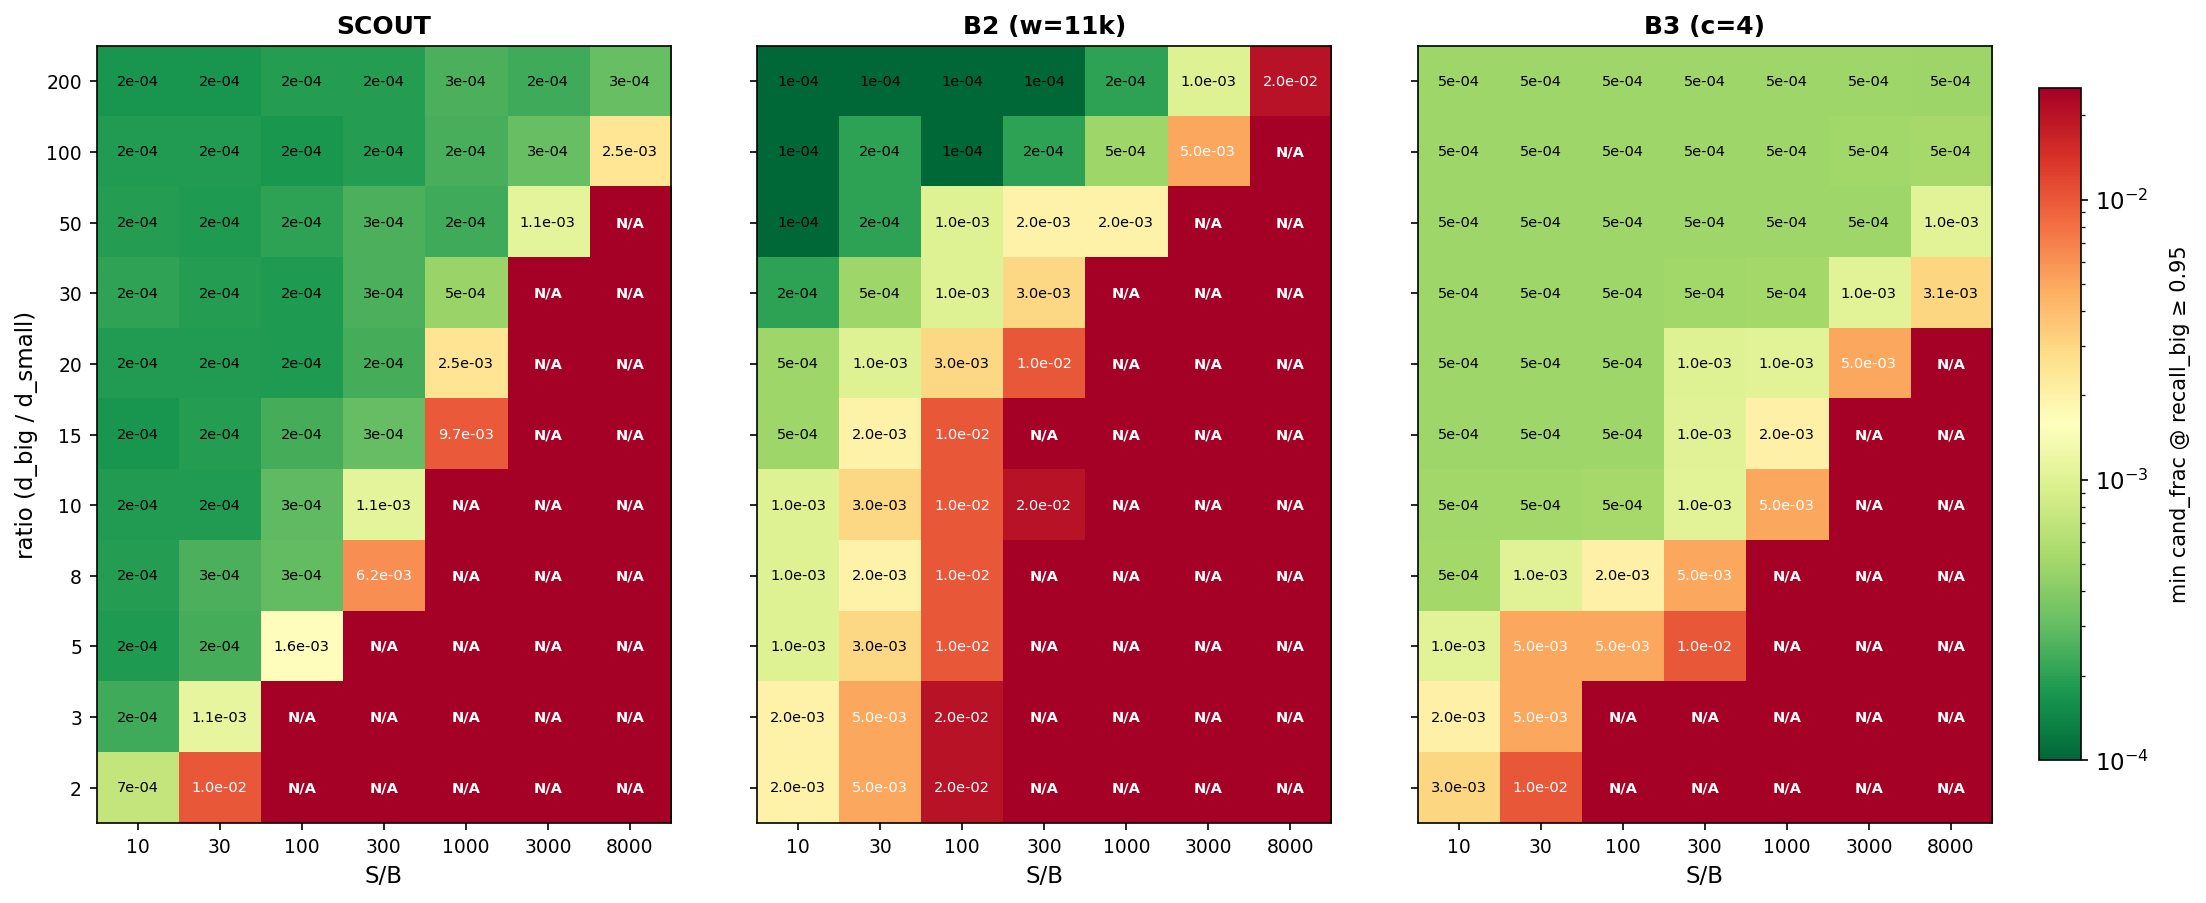
\includegraphics[width=0.9\linewidth]{figures/exp20v4_all_methods_heatmap_notitle.png}
\caption{Triage operating-point heatmap (same budget, single-round probe). Color encodes the minimum $\texttt{cand\_frac}$ achieving $\texttt{median(recall\_big)}\ge 0.95$ (log scale); N/A indicates the recall constraint cannot be met within the 2\% cap.}
\label{fig:c5-1}
\end{figure*}

We construct a family of mixed workloads with $P{=}100{,}000$ and $\texttt{total\_diff}{=}200{,}000$, comprising $B$ heavily dirty segments (each with $d_{\text{big}}$ diff keys) and $S$ noise segments (each with $d_{\text{small}}$ diff keys). The difficulty of separating heavy hitters from noise is parameterized along two axes: $\texttt{S/B}$ (noise-to-signal multiplier) and $\texttt{ratio}{=}d_{\text{big}}/d_{\text{small}}$ (separability). Figure~\ref{fig:c5-1} shows each method's feasible region on this two-dimensional parameter grid under a 2\% candidate budget cap. Greener cells indicate a lower required candidate fraction, whereas red cells marked as N/A denote configurations that cannot meet the recall constraint.

B2 degrades when heavy-tail noise collapses the per-segment ranking margin. With many noise segments (high $\texttt{S/B}$) and a small intensity gap (low $\texttt{ratio}$), mildly dirty segments flood the top-$K$ ranking and displace the genuinely heavy ones. At high separability ($\texttt{ratio}{=}200$), B2 achieves a slightly lower candidate fraction than SCOUT (${\sim}10^{-4}$ vs.\ ${\sim}2{\times}10^{-4}$), because direct ranking is highly effective when per-segment signals are already well separated; SCOUT pays a small halo cost from window aggregation. Once $\texttt{ratio}$ drops to single digits, however, B2 rapidly enters N/A. Doubling B2's memory to ${\sim}1$\,MiB does not change this picture: the low-separability region at $\texttt{ratio}\le 5$ remains unreachable (Supplement~\ref{sec:appendix-comp-triage}).

B3 is limited by the discrete granularity of its hierarchy. Once a leaf bucket is selected, the entire bucket must be expanded, so the candidate fraction increases in bucket-sized jumps rather than smoothly. Under heavy-tail noise, many buckets accumulate moderate discrepancy mass at the same time, which pushes the candidate set quickly toward the 2\% cap. An ablation over $B$ ($10{\to}100$) shows that SCOUT's feasible region shrinks by $25$\,pp, compared with $43$\,pp for B2 and $39$\,pp for B3. Additional checks, including doubling B2's memory, relaxing the candidate cap from 2\% to 5\% and 10\%, and sweeping $B$, do not change the qualitative comparison (Supplement~\ref{sec:appendix-comp-triage}).




\paragraph{Gating reliability under the same budget} \label{sec:eval-comp-gating}

\begin{figure}[!htbp]
\centering
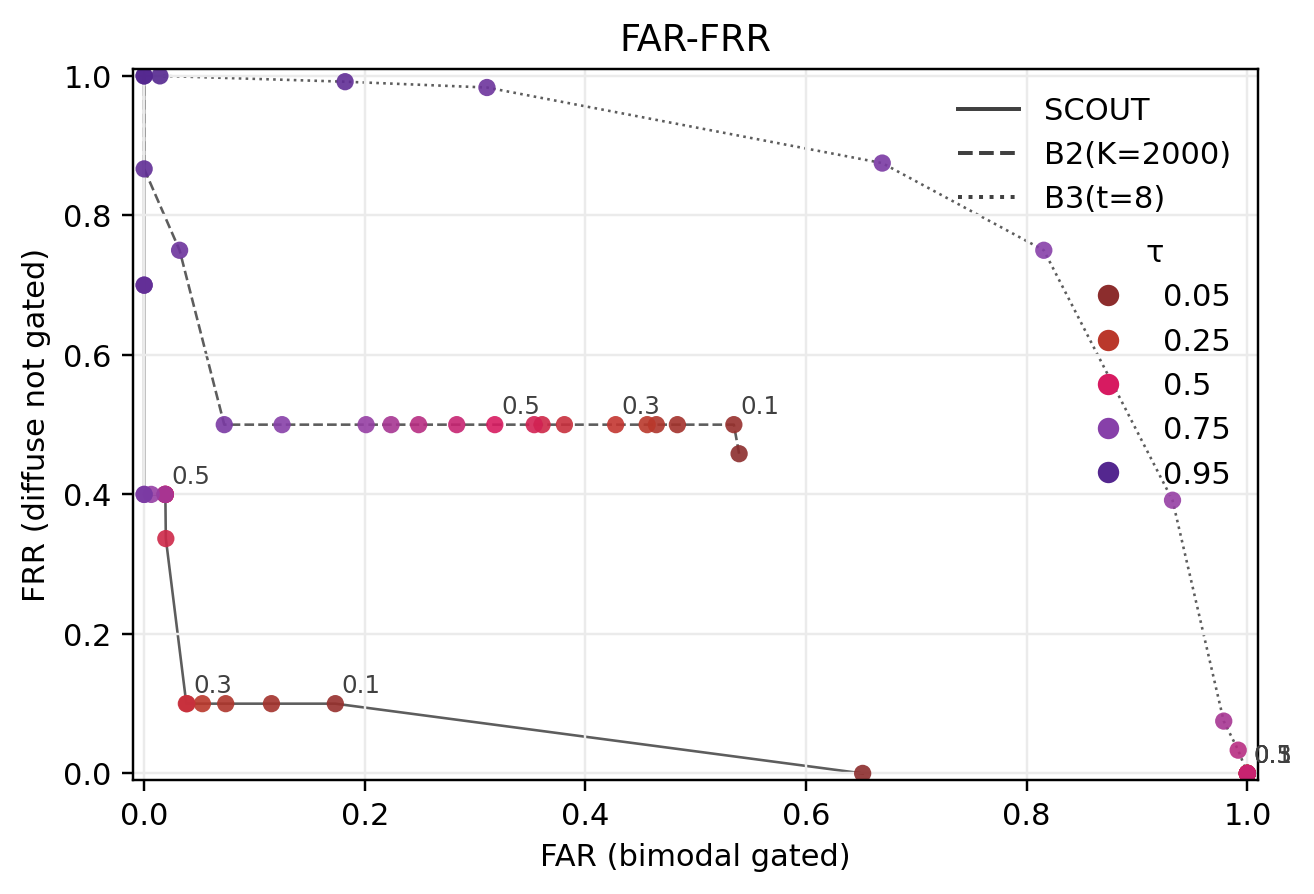
\includegraphics[width=0.92\linewidth]{figures/exp22v1_tradeoff_minT64_taulegend.png}
\caption{Conditional FAR--FRR trade-off (${\sim}512$\,KiB). Each point on a curve corresponds to a $\tau_{\text{gating}}$ threshold; the lower-left corner is the ideal region.}
\label{fig:c5-5-512}
\end{figure}

Figure~\ref{fig:c5-5-512} compares the conditional FAR--FRR trade-off of the three methods at ${\sim}512$\,KiB, treating \texttt{gate} as the positive class and conditioning on decisive (that is, non-\texttt{unknown}) samples. Full definitions, threshold sweeps, and supplementary analyses are provided in Supplement~\ref{sec:appendix-comp-gating}. SCOUT uses $K_{\text{eff}}/L$ as the gating statistic. B2 uses the fraction of total estimated mass not captured by its top-ranked segments, which stays near 0 when discrepancy mass is concentrated in a few segments and increases as the mass becomes more diffuse. B3 uses the maximum per-level fan-out ratio, using the most expanded level as a proxy for how diffusely the discrepancy spreads through the hierarchy.


\phantomsection\label{sec:eval-comp-far-frr}
Only SCOUT attains operating points with both low FAR and low FRR. Under the constraint $\texttt{FRR\_cond}\le 0.10$, $\tau_{\text{gating}}$ remains feasible across the interval $0.15$--$0.40$; at the representative point $\tau_{\text{gating}}{=}0.40$, $\texttt{FAR\_cond}\approx 0.038$ and $\texttt{FRR\_cond}{=}0.10$. The residual ${\sim}4\%$ conditional false-alarm rate is concentrated in borderline cases with high noise coverage. In contrast, B2's curve plateaus at $\texttt{FRR\_cond}{=}0.50$: regardless of threshold tuning, half of the diffuse samples are never intercepted, because heavy-tail noise dilutes concentrated faults to resemble diffuse ones, and B2's statistic cannot distinguish the two. B3 remains confined to the high-FAR, high-FRR region. Nearly all concentrated faults are misclassified as diffuse. Within shared buckets, collisions between dirty and clean segments inflate upper-level fan-out even for concentrated faults, leaving B3 with no usable trade-off interval (Supplement~\ref{sec:appendix-comp-gating}).
